%===============================================================================%
% Author: Pablo S�nchez (pablo@lcc.uma.es; http://www.lcc.uma.es/~pablo)        %
% Section : Expressing and validating ...                    Date: 25/11/2009   %
% Version : 1.0                                                                 %
% Conference: Caise 2010                                                        %
%===============================================================================%

Once we have specified a set of external constraints, we need to design a mechanism for evaluating them given a certain input configuration model, in order to decide if such a configuration model satisfies these constraints and it can, therefore, be considered a valid configuration. Moreover, if a configuration were not valid, we would like to know why it is not valid, and, if it is possible, to (semi)automatically carry out some corrective actions. The input configuration model can be a partial configuration model, i.e. a configuration model where certain features has still neither selected nor unselected. 

We can evaluate these constraints and achieve these goals by translating them into a Constraint Satisfaction Problem~\cite{tsang:1993}. A Constraint Satisfaction Problem is defined as a triple $(X, D, C)$, where $X$ is a finite set of variables, $D$ is a finite set of domains of values (one domain for each existing variable in $X$), and $C$ is set of constraints defined on $V$. Thus, we need to decide how many variables we need to create, which domain these variables will have and if we need to adapt our constraints in order to fit in with a constraint satisfaction problem.

A first tentative, is to create a variable by each potential feature, and to assign to each variable a boolean value depending on if the variable has been selected or not. Nevertheless, since clonable features can have an infinite upper bound, there might be an infinite number of variables, and the set of variables $X$ must be finite. But, it should be noticed that although a feature model can have an  infinite number of configurations, each configuration is finite, since each configuration must have, by definition, a finite number of clones. Therefore, clonable and multiple features are translated into variables of a CSP based on a (partial) configuration model, instead of a configuration model. 

The algorithm for creating the variables for the CSP is as follows. We assume that each clone has a unique name, which serves as feature identifier.

\begin{enumerate}
    \item Then, we create a variable for each simple feature in the feature model. The domain of each variable is ${true, false}$. If a feature can be univocally identified, the name of the variable is the same name as the feature. Otherwise, we preclude the name of the variable with as many name of ancestor features were required to univocally identified it. So, a feature referenced as $Facilities[LightMng]$ would be translated into a variable with name \imp{Facilities\_LightMng}
    \item For each clonable or multiple feature, we create a variable with domain ${a..b}$, where $a, b$ are positive integers, and $b$ can be infinite. These boundaries are calculated using the process that will explain below. 
    \item For each clone in the configuration model, we create a variable for each multiple feature that becomes a simple feature in the context of such a clone. The domain of each variable is ${true, false}$. The name of the variable is the same name of the feature, preclude by the name of the clone. So, the variable for the \imp{FloorFacilities} feature belonging to the \imp{GroundFloor} clone would be name as \imp{GroundFloor\_FloorFacilities}. As before, we preclude the name of the variable with as many name of ancestor features were required to univocally identified it.
    \item For each clone, we create a variable for each multiple feature that remains a multiple feature in the context of such a clone. The domain of each variable is ${a..b}$, where $a, b$ are positive integers, and $b$ can be infinite. These boundaries are calculated using the process that will explain below, but using the clone as a root for the feature model.
\end{enumerate}

%==================================================================================================================%
% NOTE(Pablo): I need to update the figure                                                                         %
%==================================================================================================================%

\begin{figure}
  % Requires \usepackage{graphicx}
  \centering 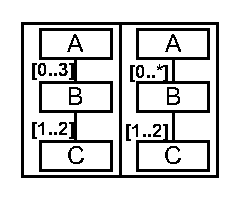
\includegraphics[width=.3\linewidth]{Figures/lowerUpperBounds.eps}\\
  \caption{Calculating lower and upper bound of clonable features}
  \label{fig:lowerUpperBounds}
\end{figure}

If a clonable feature has as cardinality ${a..b}$, it does not mean that this feature can have between $a$ and $b$ instances. See for instance Figure~\ref{fig:lowerUpperBounds} (a). Feature \imp{C} has as lower bound $1$, but it means it need to appear at least one time by each feature $B$, and there must be four clones of the feature $B$ at least. Therefore, the minimum number of clones of the feature $C$ in a whole configuration model is four. So, the global lower bound of a feature $F$ is calculated by multiplying the lower bounds of each feature in the path from such a feature $F$ to the root of the feature model. In this path, optional features are considered to have cardinality $0..1$, mandatory features $1..1$ and grouped features has the same cardinality as the feature group. So, the lower bound of feature $C$, in Figure~\ref{fig:lowerUpperBounds} (b) would be zero. Upper bounds are calculated in the same way, but multiplying the upper bounds of each features. For instance, the upper bound of $C$ in Figure~\ref{fig:lowerUpperBounds} (a) would be infinite; and for Figure~\ref{fig:lowerUpperBounds} (a) would be two.

Applying this process to the feature model of Figure~\ref{fig:smartHomeFM} and the configuration model of Figure~\ref{fig:smartHomeCfg} would be as follows:

%=============================================================================================================%
% NOTE(Pablo): Esto es un co�azo y deber�a ser reducible                                                      %
%=============================================================================================================%

\begin{enumerate}
    \item We create a variable for $SmartHome$ and $Facilities$ with domain ${true,false}$.
    \item We create the variables $Floor$, $Room$, $Devices$, $FloorFacilities$, $RoomFacilities$ with domain $[1..*]$.
    \item We create the variables $Window$, $Heater$ and $Light$, $LightMng$,
          $WindowMng$, $HeaterMng$ and $SmartEnergyMng$ with domain $[0..*]$.
    \item We create the variables $Facilities_LightMng$, $Facilities_WindowMng$, $Facilities_LightMng$ and $Facilities_SmartEnergyMng$ with domain ${true,false}$.
    \item We create the variables $GroundFloor_FloorFacilities$, $GroundFloor_FloorFacilities_WindowMng$, $GroundFloor_FloorFacilities_LightMng$ and $GroundFloor_FloorFacilities_SmartEnergyMng$ with domain ${true,false}$.
    \item We create the variables $GroundFloor_Room$, $GroundFloor_RoomFacilities$, $GroundFloor_Devices$ with domain $[1..*]$.
    \item We create the variables $GroundFloor_Window$, $GroundFloor_Heater$, $GroundFloor_Light$, $GroundFloor_LightMng$, $GroundFloor_WindowMng$, $GroundFloor_HeaterMng$ and $GroundFloor_SmartEnergyMng$ with domain $[0..*]$.
    \item We create the variables $Kitchen_RoomFacilities$, $Kitchen_RoomFacilities_WindowMng$, $Kitchen_RoomFacilities_LightMng$ and $GroundFloor_RoomFacilities_SmartEnergyMng$ with domain ${true,false}$.
    \item We create the variables $Kitchen_Window$, $Kitchen_Heater$, $Kitchen_Light$ with domain $[0..*]$.
    \item We create similar variables to steps 8 and 9, but for the \imp{Bedroom} clone.
\end{enumerate}

Then, we translate the different constraints into constraints for a CSP. For solving a CSP, we have opted for using Choco~\cite{}, a Java library for CSP, since it shows a promising performance in several CSP bechmarks~\cite{}. Choco provides logical operators plus comparison operators for specifying constraints. Thus, the problem of translating logical expressions and comparison expressions is reduced to rewriting the constraints specified in the language presented in the previous section in proper Choco syntax. For instance, the constraint \imp{C01} of Figure~\ref{fig:constraints} would be translated into a Choco constraint with the syntax, 

\begin{figure}
\begin{scriptsize}
\begin{verbatim}
    \imp{implies(Facilities\_SmartEnergy,and(Facilities\_HeaterMng,Facilities\_WindowMng))}
\end{verbatim}
\end{scriptsize}
\caption{CSP constraint for constraint \imp{C01}}
\label{eq:c01}
\end{figure}

Thus, the problem is basically reduced to the translation of context expressions with quantifiers. In this case, the solution for translating a constraint like \imp{<quantifier> <MultiValueFeature> [ Constraint ]}, is to replicate the translation of \imp{<Constraint>} as many times as clones the \imp{<MultiValueFeature>} has. The translation of \imp{<Constraint>} is performed as any other constraint, but assuming that each replica of \imp{<Constraint>} is evaluated in the context of an unique clone of such a feature, i.e. the constraint is evaluated using exclusively the subtree below that clone. Therefore, we need to replace the variables in \imp{<Constraint>} by the variables that refer to the features below the clone. If the quantifier is \imp{any}, we join all these replicas by \emph{or} relationships. If the quantifier is \imp{all}, we join all these replicas by \emph{and} relationships.  

% We denote that a constraint $C$ is evaluated using a given feature instance $FI$ as context as \imp{I \vDash C}. Thus, % for instance, using the configuration model of Figure~\ref{fig:smartHomeCfg}, $\imp{Kitchen} $\vDash$  LightMng$} 
% would be evaluated to false, whereas $\imp{Bedroom} $\vDash$ LightMng$} would be evaluated to true.

Thus, for instance, the constraint \imp{C05} in Figure~\ref{fig:constraints}, would be translated following the next process: (1) We calculate the set of clones of the feature $Floor$. In this case, $Floor = {GroundFloor}$. Thus, each feature in the internal constraint refers to a feature below $GroundFloor$; (2) Then, we translate the internal constraint, which generates a Choco constraint such as depicted in~\ref{eq:C05}.

\begin{figure}
\begin{scriptsize}
\begin{verbatim}
  implies(GroundFloor\_FloorFacilities\_SmartEnergy,      
          and(GroundFloor\_FloorFacilities\_HeaterMng,    
              GroundFloor\_FloorFacilities\_WindowMng))}  
\end{verbatim}
\end{scriptsize}
\caption{CSP constraint for constraint \imp{C05}}
\label{eq:c05}
\end{figure}

In the case of the constraint \imp{C13} in Figure~\ref{fig:constraints}, we would need to create several replicas of the constraint, and to use different sets of variables for each replica, according to the different clones of the feature \imp{Room}. The translation of such a constraint is depicted in Figure~\ref{eq:13}

\begin{figure}
\begin{scriptsize}
\begin{verbatim}
  and(implies(Kitchen\_HeaterMng,gt(Kitchen\_Heater,0)),
             implies(Bedroom\_HeaterMng,gt(Bedroom\_Heater,0))))}
\end{verbatim}
\end{scriptsize}
\caption{CSP constraint for constraint \imp{C05}}
\label{eq:c13}
\end{figure}

Finally, we need to bind the variables that have been already selected or unselected in the configuration model. For each boolean variable $v$, a constraint \imp{eq(v,true)} is added to the set of constraints if the corresponding feature has been selected; otherwise, a constraint \imp{eq(v,false)} is added to such a set. For each integer variable representing a clonable or multiple feature, the number of clones is calculated and that variable initialized to that number of clones. 

Once we have defined our CSP, we can solve using a third-party library as Choco. Choco calculates if the current configuration satisfies the external constraints, and if it is not so, it provides information about what constraints has been violated. Moreover, Choco can be used to perform some kind of useful analysis on partial configurations. 

For instance, given an invalid partial configuration, Choco can use constraint propagation to calculate what features should be added to the current configuration in order to create a valid configuration. We can also Choco to complete a configuration given a certain criteria. 

For instance, let us suppose we have the configuration model of Figure~\ref{fig:smartHomeCfg}, but \imp{WindowMng} has not been selected neither at the \imp{Floor} nor at the \imp{Room} level (and it has been selected at the house level). But, according to constraints \imp{C02} and \imp{C07}, it should have been also selected at the floor and room levels. Using constraint propagation, Choco can calculate that these features are lacking at these levels, and \emph{Hydra}, our feature modelling tool, would add them to the configuration model.

If, given a partial configuration, this can be completed in several ways, we can use Choco to select the configuration, which fulfill some kind of arbitrary criteria, such as having the lower number of features. 




% In our case, $V$ would be the features contained in the feature model. Each simple feature is transformed into a
% variable $v \in V$, with domain $D_{i} = {TRUE, FALSE}$. Each clonable and multiple feature is transformed into a
% variable $v \in V$ with domain $D_{i} = {a..b}$, where $a$ is the minimum number of times the clonable feature can
% appear in a feature diagram and $b$ the upper bound. These limits do not necessarily need to be the limits of the
% clonable feature. See for instance, Figure~\ref{fig:lowerUpperBounds} (a). Feature \imp{D} has as lower bound $1$, but % it means it need to appear $1$ time by each feature $B$, and there must be $4$ clones of the feature $B$ at least.
% Therefore, the minimum number of clones of the feature $D$ in a whole configuration model is $4$. The global lower
% bound of a feature $F$ is calculated by multiplying the lower bounds of each feature in the path from such a feature
% $F$ to the root of the feature model. In this path, optional features are considered to have cardinality $0..1$,
% mandatory features $1..1$ and grouped features has the same cardinality as the feature group. Upper bounds are
% calculated in the same way, but multiplying the upper bounds of each features. It should be noticed that any $0$ in
% the lower bound of the features in that path means the lower bound will be zero, and any $*$ in the upper bounds means % that the upper bound will be $*$. Then, for each clone in the feature model we create a variable $v \in V$. We do not % consider clones the selections of simple features. These variables has as domain ${TRUE}$, it is said, they always
% evaluate to true since
% they already exist in the configuration model.

